\let\negmedspace\undefined
\let\negthickspace\undefined
\documentclass[journal]{IEEEtran}
\usepackage[a5paper, margin=10mm, onecolumn]{geometry}
%\usepackage{lmodern} % Ensure lmodern is loaded for pdflatex
\usepackage{tfrupee} % Include tfrupee package

\setlength{\headheight}{1cm} % Set the height of the header box
\setlength{\headsep}{0mm}     % Set the distance between the header box and the top of the text
\usepackage{multicol}
\usepackage{gvv-book}
\usepackage{gvv}
\usepackage{cite}
\usepackage{amsmath,amssymb,amsfonts,amsthm}
\usepackage{algorithmic}
\usepackage{graphicx}
\usepackage{textcomp}
\usepackage{xcolor}
\usepackage{txfonts}
\usepackage{listings}
\usepackage{enumitem}
\usepackage{mathtools}
\usepackage{gensymb}
\usepackage{comment}
\usepackage[breaklinks=true]{hyperref}
\usepackage{tkz-euclide} 
\usepackage{pgfplots}
\pgfplotsset{compat=1.18}
\usepackage{listings}
% \usepackage{gvv}                                        
\def\inputGnumericTable{}                                 
\usepackage[latin1]{inputenc}                                
\usepackage{color}                                            
\usepackage{array}                                            
\usepackage{longtable}                                       
\usepackage{calc}                                             
\usepackage{multirow}                                         
\usepackage{hhline}                                           
\usepackage{ifthen}                                           
\usepackage{lscape}
\usepackage{tikz}
% Marks the beginning of the document
\begin{document}
\bibliographystyle{IEEEtran}
\vspace{3cm}

\title{Finding maximum value\\NCERT-12.6.5.24}
\author{EE24BTECH11056 - S.Kavya Anvitha}
\maketitle
%\newpage
\bigskip

\renewcommand{\thefigure}{\theenumi}
\renewcommand{\thetable}{\theenumi}
\textbf{Question:}\\
Our aim is to find the maximum value of the function:
\begin{align}
    f(x) = \left[ x(x-1) + 1 \right]^{1/3}
\end{align}
in the interval $0\leq x \leq 1$ using the gradient ascent method\\
Simplify the expression 
\begin{align}
    f(x) = \left[ x^2 - x + 1 \right]^{1/3}
\end{align}
Letting , the derivative of  using the chain rule is:
\begin{align}
f'(x) = \frac{d}{dx} \left( g(x)^{1/3} \right) = \frac{1}{3}g(x)^{-2/3} \cdot g'(x),
\text{where:}
g'(x) = 2x - 1
\end{align}
The gradient ascent update rule is:
\begin{align}
x_{n+1} = x_n + \eta \cdot f'(x_n)
\end{align}
where:\\
\begin{enumerate}
    \item $x_n$ is the current estimate.
    \item $\eta$ is the learning rate.
    \item $f'(x) $ is the derivative calculated above.
\end{enumerate}
Implementing gradient ascent:
\begin{enumerate}
    \item We need to Choose a small learning rate $\eta$ (say, 0.01).
    \item Choose a starting point $x_0$ (say 0.0)
\end{enumerate}
Compute the gradient $f'(x_n)$\\
Update the current point using the formula 
\begin{align}
x_{n+1} = x_n + \eta \cdot f'(x_n)\\
x_{n+1} = x_n + \eta \cdot \frac{1}{3}([x_n^2-x_n+1]^{\frac{-2}{3}})\cdot\brak{2x_n-1}
\end{align}
For finding minimum we use gradient descent method.Update the value of $x$ using the formula:\\
\textbf{gradient descent update rule is:}
\begin{align}
  x_{n+1} = x_n - \eta \cdot f'(x_n)\\
x_{n+1} = x_n - \eta \cdot \frac{1}{3}([x_n^2-x_n+1]^{\frac{-2}{3}})\cdot\brak{2x_n-1}
\end{align}
Check if the stopping condition is met.\\
The value of $x$ after sufficient iterations will be the approximate point where the function attains its minimum.\\
\textbf{Behavior in each region:}\\
for $x>0.5$ : $g'(x) = 2x - 1>0$\\
for $x<0.5$ : $g'(x) = 2x - 1<0$\\
Stop when the gradient is close to zero(e.g.,$\abs{f'(x_n)}< 10^{-6}$)\\
Stop if the next step takes $x$ out of the interval [0,1].\\
Since the interval is restricted to $0\leq x \leq 1$:\\
\begin{enumerate}
    \item Compute the function value at the boundaries $f(0)$ and $f(1)$.
    \item Compare with the value obtained using gradient ascent.
\end{enumerate}
\textbf{Boundary values:}\\
$f(0) = [0(0-1)+1]^{\frac{1}{3}} = 1$\\
$f(1) = [1(1-1)+1]^{\frac{1}{3}} = 1$
\begin{figure}[h!]
   \centering
   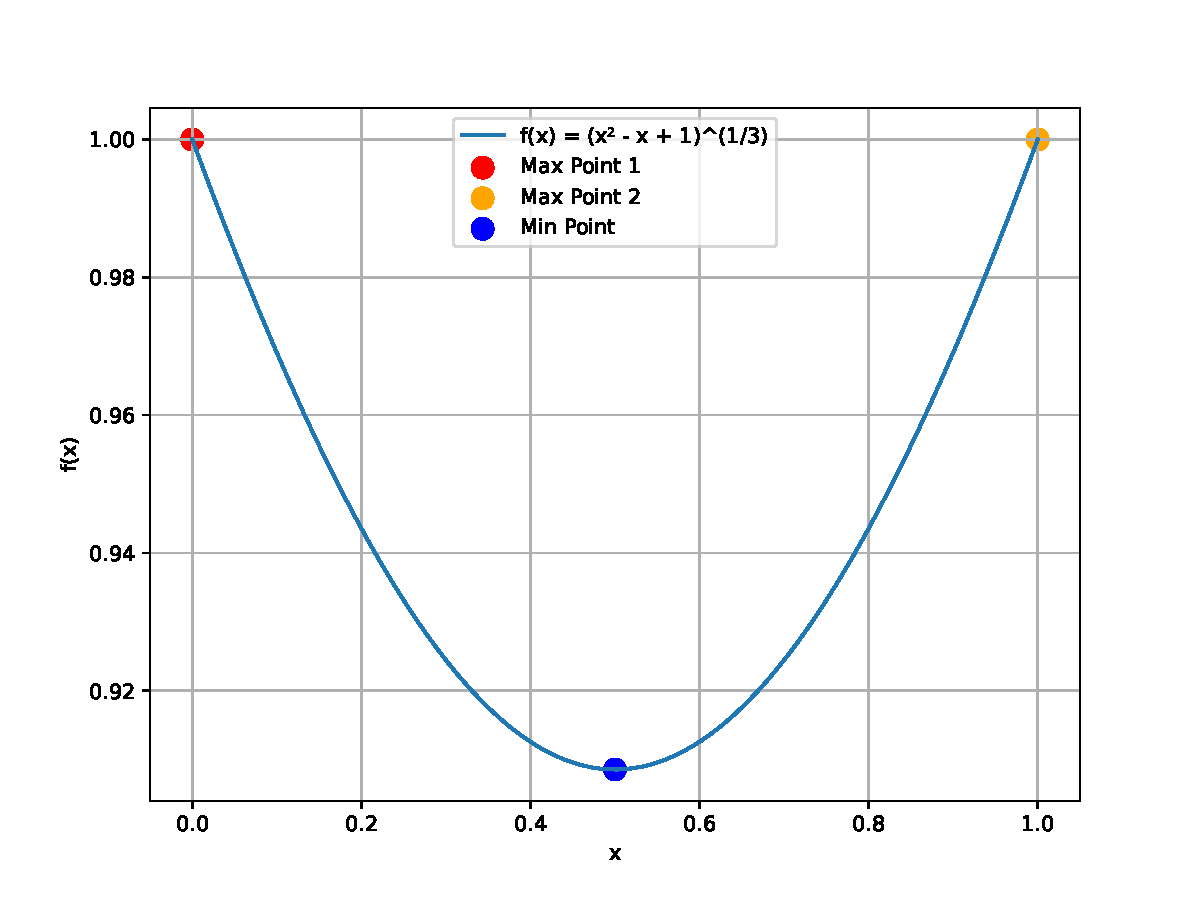
\includegraphics[width=\columnwidth]{figs/fig.pdf}
\end{figure}
\end{document}
